\hyphenation{аудио-драмах}
\hyphenation{аудио-записях}

\chapter{Аниме: загадочный и поразительный мир японской анимации}
\label{ch:anime}
%
\marginnote[0.0cm]{Сэйю~--- это японские актёры озвучивания. Сэйю обычно озвучивают роли персонажей в аниме, видеоиграх, фильмах, а также на радио и телевидении, или выступают в роли рассказчика в радиопостановках. Кроме того, голоса сэйю используются в рекламе, голосовых объявлениях, аудиозаписях книг и учебных материалов, а также для переозвучивания. Сэйю могут быть как мужчины, так и женщины; как взрослые, так и дети.}

В рамках этой главы исследуется объект Викиданных \wdqName{<<аниме>>}{1107}. С помощью SPARQL-запросов, вычисляемых на объектах типа <<аниме>> в Викиданных, получен список сэйю, упорядоченный по числу озвученных ими аниме, построен график числа аниме, озвученных одним сэйю, построен граф, связывающий сэйю и озвученные ими аниме, получена оценка трудоспособного возраста сэйю. 

\begin{marginfigure}[0.0cm]
{
	\setlength{\fboxsep}{0pt}%
	\setlength{\fboxrule}{1pt}%
	\fcolorbox{gray}{gray}{
\includegraphics[width=0.5\linewidth]{chapter/anime/seyu.jpg}}
}
\caption
[Сэйю Кэндзи Акабанэ.]%
{%
Сэйю Кэндзи Акабанэ озвучивал роль персонажа Sasuke Sarutobi в видеоигре Ikemen Sengoku, 2018 год.\newline
Wikimedia Commons / numan (CC BY-SA)
}
\label{fig:seiyu}
\end{marginfigure}

\section{Экземпляры объекта <<Аниме>>}

Аниме~--- это японская мультипликация. Она стоит особняком и выделяется своим визуальным стилем, однако есть и менее очевидные отличия: так, по сравнению с американской и японской анимацией у аниме значительно шире список жанров~--- от детских и семейных комедий до драматических историй, которые на Западе обычно изображаются только в фильмах с живыми актёрами\autocite{anime_vs_animation}.

У каждого аниме есть свои актёры озвучивания. В дальнейшем под <<сэйю>> будем понимать японского актёра озвучивания. В японской анимации слова <<актёры озвучивания>> и <<сэйю>> являются синонимами\autocite{shikimori}. Под словом <<тайтл>> (от англ. \emph{title}, \emph{название}) обычно понимают конкретное аниме\autocite{anime_social}. В общем же смысле слово <<тайтл>> означает понятие, объединяющее различные виды продукции (от кинофильма до романа), созданные на основе конкретного произведения, за которым закреплено строго определённое название\autocite{anime_title_def}.

Чтобы работать со списком аниме в Викиданных, нам понадобятся объект \wdqName{<<аниме>>}{1107} и свойство \wdProperty{31}{<<экземпляр>>}. Получим список всех аниме без учёта подклассов (листинг~\ref{lst:anime}).

\newpage

\begin{lstlisting}[ language=SPARQL, 
                    caption={\href{https://w.wiki/4ABw}{Список аниме без учёта подклассов}\protect\footnotemark},
                    label=lst:anime,
                    texcl,
                    numbers=none,
                    ]
# List of instances of anime
SELECT ?anime ?animeLabel
WHERE
{
    ?anime wdt:P31 wd:Q1107. # instance of anime
    SERVICE wikibase:label{bd:serviceParam wikibase:language "ru,en,ja"}
}
\end{lstlisting}%
\footnotetext{Получено \num{683} результата в 2017 году и \num{216} результатов в 2021 году. Ссылка на SPARQL-запрос: \href{https://w.wiki/4ABw}{https://w.wiki/4ABw}}

\begin{marginfigure}[1\baselineskip]
{
	\setlength{\fboxsep}{0pt}%
	\setlength{\fboxrule}{1pt}%
	\fcolorbox{gray}{gray}{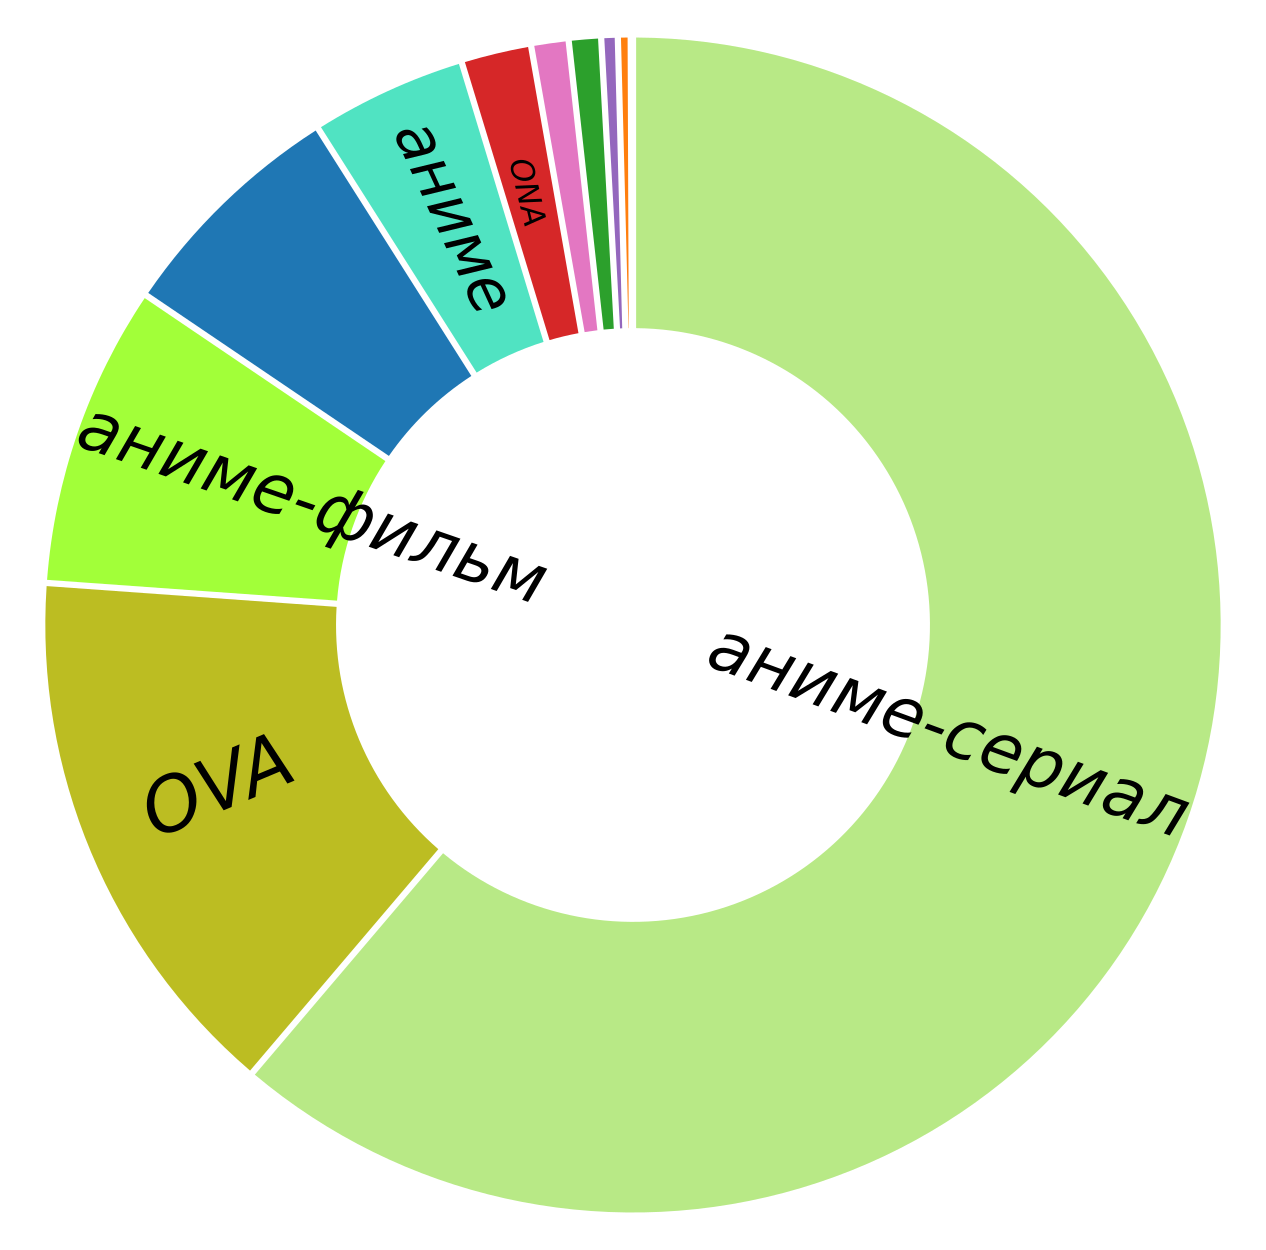
\includegraphics[width=0.5\linewidth]{chapter/anime/anime-subclasses-sunburst-diagram-2021.png}}
}
\caption%
[Жанры аниме на круговой диаграмме, 2021 год.\index{Сервисы для анализа данных!Сервисы для визуализации данных!Rawgraphs}]%
{%
Диаграмма <<солнечные лучи>>\index{График!Sunburst diagram!Количество аниме по жанрам} (sunburst diagram) жанров аниме, построенная с помощью сервиса Rawgraphs (\href{https://app.rawgraphs.io}{https://app.rawgraphs.io}).\newline
}%
\label{fig:anime_piechart}
\end{marginfigure}

В действительности в Викиданных объектов аниме гораздо больше, но они являются экземплярами не объекта <<аниме>>, а его подклассов, таких как, например, \wdqName{<<аниме-сериал>>}{63952888}. Чтобы получить список жанров аниме и количество аниме, относящихся к этим жанрам, выполним другой запрос (листинг~\ref{lst:anime_w_subclass}).

\begin{lstlisting}[ language=SPARQL, 
                    caption={\href{https://w.wiki/4ABj}{Список жанров аниме и количество аниме, относящихся к этим жанрам}\protect\footnotemark},
                    label=lst:anime_w_subclass,
                    numbers=none,
                    texcl 
                    ]
# Select anime and its subclasses with number of titles
# corresponding to these subclasses
SELECT ?subAnime ?subAnimeLabel (COUNT(?subAnimeInst) AS ?count)
WHERE {
  ?subAnime wdt:P279* wd:Q1107.   # select anime subclass list
  ?subAnimeInst wdt:P31 ?subAnime # link titles and subclasses
    SERVICE wikibase:label{bd:serviceParam wikibase:language "ru,en,ja"}
}
GROUP BY ?subAnime ?subAnimeLabel
ORDER BY DESC(?count)
\end{lstlisting}%
\footnotetext{Получено \num{11} результатов в 2021 году. Ссылка на SPARQL-запрос: \href{https://w.wiki/4ABj}{https://w.wiki/4ABj}}

Визуализировать распределение аниме по жанрам можно с помощью, например, диаграммы <<солнечные лучи>> (рис.~\ref{fig:anime_piechart})\index{Сервисы для анализа данных!Сервисы для визуализации данных!Rawgraphs}.

Полученная классификация аниме по жанрам не идеальна, так как есть большое смещение в сторону аниме-сериалов: из \num{4875} тайтлов \num{2984} отнесены к жанру <<аниме-сериал>> (\num{62,7}\%); вероятно, классификация жанров аниме в Викиданных требует дальнейшего уточнения. Также в подклассы попали понятия, относящиеся не к общей классификации, а к отдельным аниме, например, \href{https://w.wiki/4L5p}{<<Евангелион>>}.

\newpage
Получим список всех аниме, включая тайтлы, относящиеся к жанрам аниме (листинг~\ref{lst:all_anime_list}).

%\begin{minipage}{\linewidth}
\begin{lstlisting}[ language=SPARQL, 
                    caption={\href{https://w.wiki/49zY}{Список всех аниме в Викиданных}\protect\footnotemark},
                    label=lst:all_anime_list,
                    numbers=none,
                    texcl 
                    ]
# List of instances of anime and subclasses of anime
SELECT ?anime ?animeLabel
WHERE
{
    ?anime wdt:P31/wdt:P279* wd:Q1107. # instance of anime/subclass
    SERVICE wikibase:label{bd:serviceParam wikibase:language "ru,en,ja"}
}
\end{lstlisting}%
\footnotetext{Получено \num{683} результата в 2017 году и \num{4875} результатов в 2021 году. Ссылка на SPARQL-запрос: \href{https://w.wiki/49zY}{https://w.wiki/49zY}}
%\end{minipage}

Аниме, о которых есть наиболее полная информация на Викиданных~--- это \wdqName{Гуррен-Лаганн}{4277}, \wdqName{Space Battleship Yamato}{4292}, \wdqName{Project A-ko}{4316}. Аниме с малоинформативными записями на Викиданных оказались \wdqName{Doraemon}{711311}, \wdqName{The Animal Conference on the Environment}{97195557}, \wdqName{Assassins Pride}{96737300}.

Среди всех аниме-тайтлов в Викиданных больше всего свойств по данным сервиса ProWD\autocite{anime_prowd} у \wdqName{Fullmetal Alchemist: The Sacred Star of Milos}{1004318}\footnote{<<Стальной алхимик: Священная звезда Милоса>>~--- полнометражный аниме-фильм, являющийся продолжением аниме-сериала <<Стальной алхимик>>. Его главные герои~--- это братья-алхимики, использующие свои магические способности для борьбы с силами зла и противостояния преступникам.} (\num{24} свойства).



\subsection{Список сэйю, упорядоченный по числу озвученных ими аниме}

Разумеется, в большинстве аниме участвует не один, а множество персонажей. Соответственно, разных персонажей озвучивают разные сэйю. Большинство сэйю озвучили за свою карьеру несколько тайтлов, а многие~--- несколько десятков тайтлов. Талантливых сэйю приглашают озвучивать сразу несколько персонажей в одном аниме. Одним из самых популярных сэйю является \href{https://w.wiki/4L5q}{Хироси Камия}, имеющий множество наград и озвучивший более 180 аниме. Самым известным аниме с его участием является \href{https://w.wiki/4L5r}{<<Атака титанов>>}, где он озвучил одного из главных персонажей~--- капитана Леви.

Построим упорядоченный список сэйю по числу озвученных ими аниме (листинг~\ref{lst:seiyu_titles_sorted}).

\newpage
\begin{lstlisting}[ language=SPARQL, 
                    caption={\href{https://w.wiki/4Xph}{Упорядоченный список сэйю по числу озвученных ими аниме}\protect\footnotemark},
                    label=lst:seiyu_titles_sorted,
                    numbers=none,
                    texcl 
                    ]
# Ordered list of actors (seiyu) according to the number of anime where they took part in
SELECT ?seiyu ?seiyuLabel (COUNT(?anime) AS ?count)
WHERE
{
  ?anime wdt:P31/wdt:P279* wd:Q1107;  # instance of anime/subclass
         wdt:P725 ?seiyu.  # instance of seiyu (voice actor)
  SERVICE wikibase:label { bd:serviceParam wikibase:language "ru,en,ja" }
}
GROUP BY ?seiyu ?seiyuLabel  # group by seiyu 
ORDER BY DESC(?count)  # order by count of voiced anime
\end{lstlisting}%
\footnotetext{Получено \num{148} результатов в 2017 году и \num{2910} результатов в 2021 году. Ссылка на SPARQL-запрос: \href{https://w.wiki/4Xph}{https://w.wiki/4Xph}}



\subsection{График по числу сэйю, озвучивших одно и более аниме}

Было бы интересно построить график (линейную диаграмму) сэйю, озвучивших аниме. Чем больше аниме озвучил сэйю, тем правее на диаграмме он будет находиться. Сделать это можно с помощью скрипта~\ref{lst:seiyu_titles_graph}.

\begin{fullwidth}
%\begin{minipage}
%\lstset{numbers=left, firstnumber=1, frame=single}
\footnotetext[11]{Получено 13 результатов в 2017 году и 58 результатов в 2021 году. Ссылка на SPARQL-запрос: \href{https://w.wiki/4JvT}{https://w.wiki/4JvT}}
\begin{lstlisting}[ language=SPARQL, 
                    caption={\href{https://w.wiki/4JvT}{Построение графика по числу сэйю, озвучивших одно и более аниме}\protect\footnotemark},
                    label=lst:seiyu_titles_graph,
                    texcl 
                    ]
# Graph of the number of voice actings of different seiyu
#defaultView:LineChart
SELECT ?seiyuRoles (COUNT(?seiyuRoles) AS ?quantity) WHERE {
  FILTER(?seiyuRoles < 71) # limit the output as there are few seiyu that act in more than 71 anime
  {
     SELECT (COUNT(?seiyu) AS ?seiyuRoles) WHERE {        # count quantity of voice acting by one seiyu
       ?anime wdt:P31/wdt:P279* wd:Q1107;                 # instance of anime and its subclasses
                 wdt:P725 ?seiyu.                         # instance of seiyu
       SERVICE wikibase:label { bd:serviceParam wikibase:language "ru,en,ja"}
     }
     GROUP BY ?anime              # group list by number of voiced anime
     ORDER BY DESC(?seiyuRoles)   # order by voice acting quantity (descending)
  }
}
GROUP BY ?seiyuRoles
ORDER BY DESC(?seiyuRoles)  # grouping and sorting seiyu by number of voice actings
\end{lstlisting}%
%\lstset{numbers=none}
%\end{minipage}
\end{fullwidth}


По рис.~\ref{fig:Seiyu_num_chart_2021_ru} очевидно, что чем выше планка количества озвученных аниме, тем меньше сэйю достигают этой планки. В \num{4} строке скрипта~\ref{lst:seiyu_titles_graph} установлено ограничение в \num{71} аниме, поскольку сэйю, которые отметились в большем количестве аниме, единицы, и расширение графика вправо было бы не слишком информативным.

Многие сэйю, как показано на диаграмме~\ref{fig:Seiyu_num_chart_2021_ru}, озвучили только одно аниме~--- на графике их оказалось \num{254}. Однако сэйю~--- это профессия, которой люди зачастую посвящают всю свою жизнь. То, что, согласно Викиданным, человек за многие годы принял участие в озвучке только одного аниме, может быть связано с отсутствием информации о других его ролях в Викиданных. 

\index{График!LineChart!Число сэйю, озвучивших одно и более аниме}
\begin{figure*}[h]

    \setlength{\fboxsep}{0pt}%
    \setlength{\fboxrule}{1pt}%
    \fcolorbox{gray}{gray}{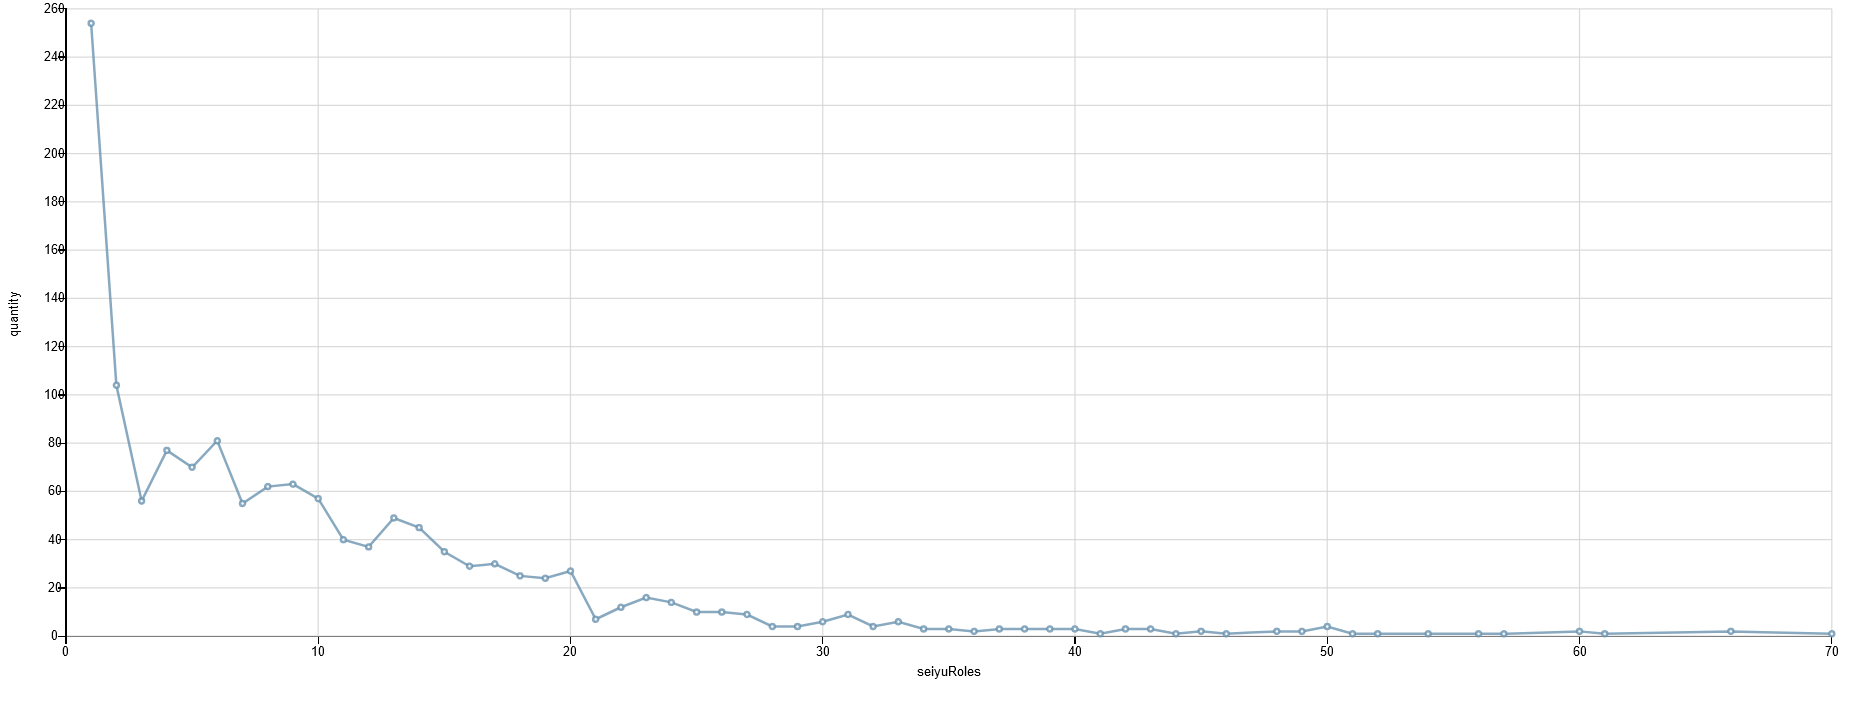
\includegraphics[width=\linewidth]{./chapter/anime/Seiyu_chart_2021_ru.png}}
	\caption[График числа ролей, озвученных различными сэйю, 2021 год.]{График числа ролей, озвученных различными сэйю, 2021 год. График построен на~основе данных, полученных с~помощью запроса~\protect\ref{lst:seiyu_titles_graph}.}%
    \label{fig:Seiyu_num_chart_2021_ru}%
\end{figure*} 

\subsection{Граф, связывающий сэйю и озвученные ими аниме}

Итак, многие сэйю за свою карьеру успевают озвучить несколько аниме. 
Чтобы нагляднее показать эту взаимосвязь, 
построим граф, связывающий сэйю и озвученные ими аниме с помощью скрипта~\ref{lst:seiyu_graph}. 
Фрагмент итогового графа представлен на рис.~\ref{fig:Seiyu_graph_2021_ru}. 


\lstset{numbers=left, firstnumber=1, frame=single}
\begin{lstlisting}[ language=SPARQL, 
                    caption={\href{https://w.wiki/4HFt}{Построение графа, связывающего сэйю и озвученные ими аниме}\protect\footnotemark},
                    label=lst:seiyu_graph,
                    texcl 
                    ]
# Graph of seiyu with more than one anime
#defaultView:Graph
SELECT DISTINCT ?item ?itemLabel ?rgb ?link
WHERE
{ # voice actors (seiyu) with more than one anime
  VALUES ?toggle { true false }
  VALUES ?seiyu { wd:Q6381410 wd:Q1347031 wd:Q1207010 
                  wd:Q233902  wd:Q1323728 wd:Q2440809 
                  wd:Q355173  wd:Q957795  wd:Q50033}
  ?anime  wdt:P31/wdt:P279* wd:Q1107; # instance of anime/subclass
          wdt:P725 ?seiyu;            # seiyu who voiced this anime 
  SERVICE wikibase:label{bd:serviceParam wikibase:language "ru,en,ja"}
  BIND(IF(?toggle,?anime,?seiyu) AS ?item).
  BIND(IF(?toggle,?animeLabel,?seiyuLabel) AS ?itemLabel).
  BIND(IF(?toggle,"FFFFFF","7FFF00") AS ?rgb).
  BIND(IF(?toggle,"",?anime) AS ?link).
}
\end{lstlisting}%
\footnotetext{Получено \num{826} результатов в 2017 году и \num{494} результата в 2021 году. Ссылка на SPARQL-запрос: \href{https://w.wiki/4HFt}{https://w.wiki/4HFt}}
\lstset{numbers=none}

В переменную \lstinline|?seiyu| (строки 7--9 запроса~\ref{lst:seiyu_graph}) записан массив объектов Викиданных, 
соответствующих некоторым известным сэйю~--- \wdqName{Кадзуэ Комия}{6381410} и другим. 
Мы выбрали только девять сэйю в иллюстративных целях, поскольку для большего числа сэйю граф стал бы неудобным для восприятия.

\index{SPARQL!BIND!Граф, связывающий сэйю и озвученные ими аниме}
\index{SPARQL!IF!Граф, связывающий сэйю и озвученные ими аниме}
Конструкция \lstinline|BIND(IF(?toggle, ?anime, ?seiyu)...)| в строке \num{13} 
позволяет определить тип вершины графа: 
если \lstinline|?toggle| принимает значение \lstinline|true|, 
то вершина графа соответствует аниме, иначе~--- сэйю. 
В строках 14 и 15 определяются тип подписи для вершины и цвет вершины. 
Строка 16 позволяет отобразить связи между сэйю и аниме.

\newpage
\begin{figure*}[h!]
    \index{График!Graph!Фрагмент графа, связывающего сэйю и озвученные ими аниме}
	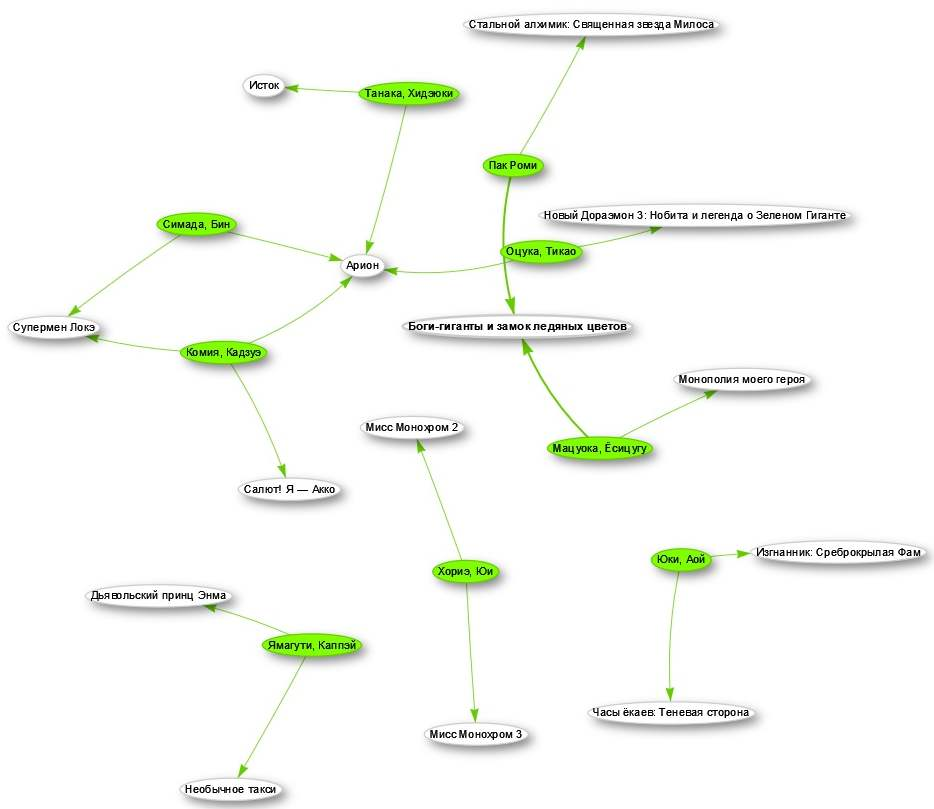
\includegraphics[width=0.7\linewidth]{./chapter/anime/Seiyu_graph_2021_ru.jpg}
	\caption[Граф сэйю и аниме, 2021 год.]{Фрагмент графа, связывающего сэйю и озвученные ими аниме, 2021. Граф построен на основе данных, полученных с помощью запроса~\protect\ref{lst:seiyu_graph}.}%
      \label{fig:Seiyu_graph_2021_ru}%
\end{figure*} 



\section{Полнота Викиданных}

Список тайтлов в \href{https://w.wiki/4JVE}{Русской Википедии}\footnote{Проект:Аниме и манга/Списки/Список аниме. \href{https://w.wiki/4JVE}{https://w.wiki/4JVE}, 2021} содержит \num{1638} аниме. Также можно посмотреть \href{https://w.wiki/4JVH}{телевизионные показы аниме в России по годам}\footnote{Проект:Аниме и манга/Телевизионные показы аниме в России по годам. \href{https://w.wiki/4JVH}{https://w.wiki/4JVH}, 2021}.

На сайте любительской энциклопедии аниме Shikimori\autocite{shikimori} в списке аниме \num{801} страница по \num{20} наименований. Нетрудно подсчитать, что на сайте есть информация о \num{16020} тайтлах, в то время как в Викиданных объектов, описывающих аниме, всего \num{4875} (см. листинг~\ref{lst:all_anime_list}). К тому же, стоит учитывать, что скорость выхода новых аниме довольно велика\footnote{Упражнение: с помощью SPARQL подсчитайте, сколько аниме вышло за прошлый год.}. Из этого можно сделать вывод, что Викиданные крайне неполно отражают данные (есть информация только о \num{29.6}\% аниме). То же самое касается и жанров: в \href{https://shikimori.one/animes}{разделе поиска Shikimori}\footnote{Лучшие аниме. \href{https://shikimori.one/animes}{https://shikimori.one/animes}, 2021} доступны \num{42} жанра аниме, в то время как Викиданные содержат информацию только о \num{17}\footnote{Список жанров (категорий) аниме, указанных в Викиданных, можно посмотреть на странице \href{https://en.wikipedia.org/wiki/Category:Lists\_of_anime\_by\_genre}{Category:Lists of anime by genre}.}.

Возможно, приведённые ниже статьи и сайты не будут являться \href{https://w.wiki/3u9v}{АИ}\footnote{Авторитетный источник (АИ)~--- это ресурс, который владеет информацией, в компетентности и актуальности которой не может быть никаких сомнений. См. \href{https://w.wiki/3u9v}{https://w.wiki/3u9v}}, но с их помощью можно проанализировать информацию об имеющихся аниме и сделать дополнительные выводы о неполноте Викиданных.

\begin{itemize}
	\item На сайте любительской озвучки \href{http://online.anidub.best/}{AniDub}\footnote{АниДаб. \href{http://online.anidub.best/}{http://online.anidub.best/}, 2021} приведён список из \num{5756} аниме.
	\item На сайте онлайн-кинотеатра \href{http://animespirit.tv/}{AnimeSpirit}\footnote{AnimeSpirit. \href{http://animespirit.tv/}{http://animespirit.tv/}, 2021} приведён список из \num{1968} аниме.
	\item На новостном форуме по тематике аниме \href{http://animeland.su/}{AnimeLand}\footnote{AnimeLand. \href{http://animeland.su/}{http://animeland.su/}, 2021} приведён список из \num{4795} аниме.
	\item На сайте онлайн-кинотеатра \href{https://anivost.org/}{Anivost}\footnote{Anivost. \href{https://anivost.org/}{https://anivost.org/}, 2021} приведён список из \num{420} аниме.
\end{itemize}

Какие-то сайты появились позже, какие-то раньше, поэтому количество аниме на них может разниться, причём довольно серьёзно. Если упорядочить все приведённые сайты, данные Русской Википедии, Английской Википедии и Викиданные по количеству аниме, то Викиданные окажутся не на последнем месте, но, например, вышеупомянутой энциклопедии \href{https://shikimori.one/}{Shikimori} они уступают почти в 4 раза.

\newpage

\noindent\begin{marginfigure}%
{%
\index{График!Sunburst diagram!Количество ролей, озвученных разными актёрами}%
\setlength{\fboxsep}{0pt}%
\setlength{\fboxrule}{1pt}%
\fcolorbox{gray}{gray}{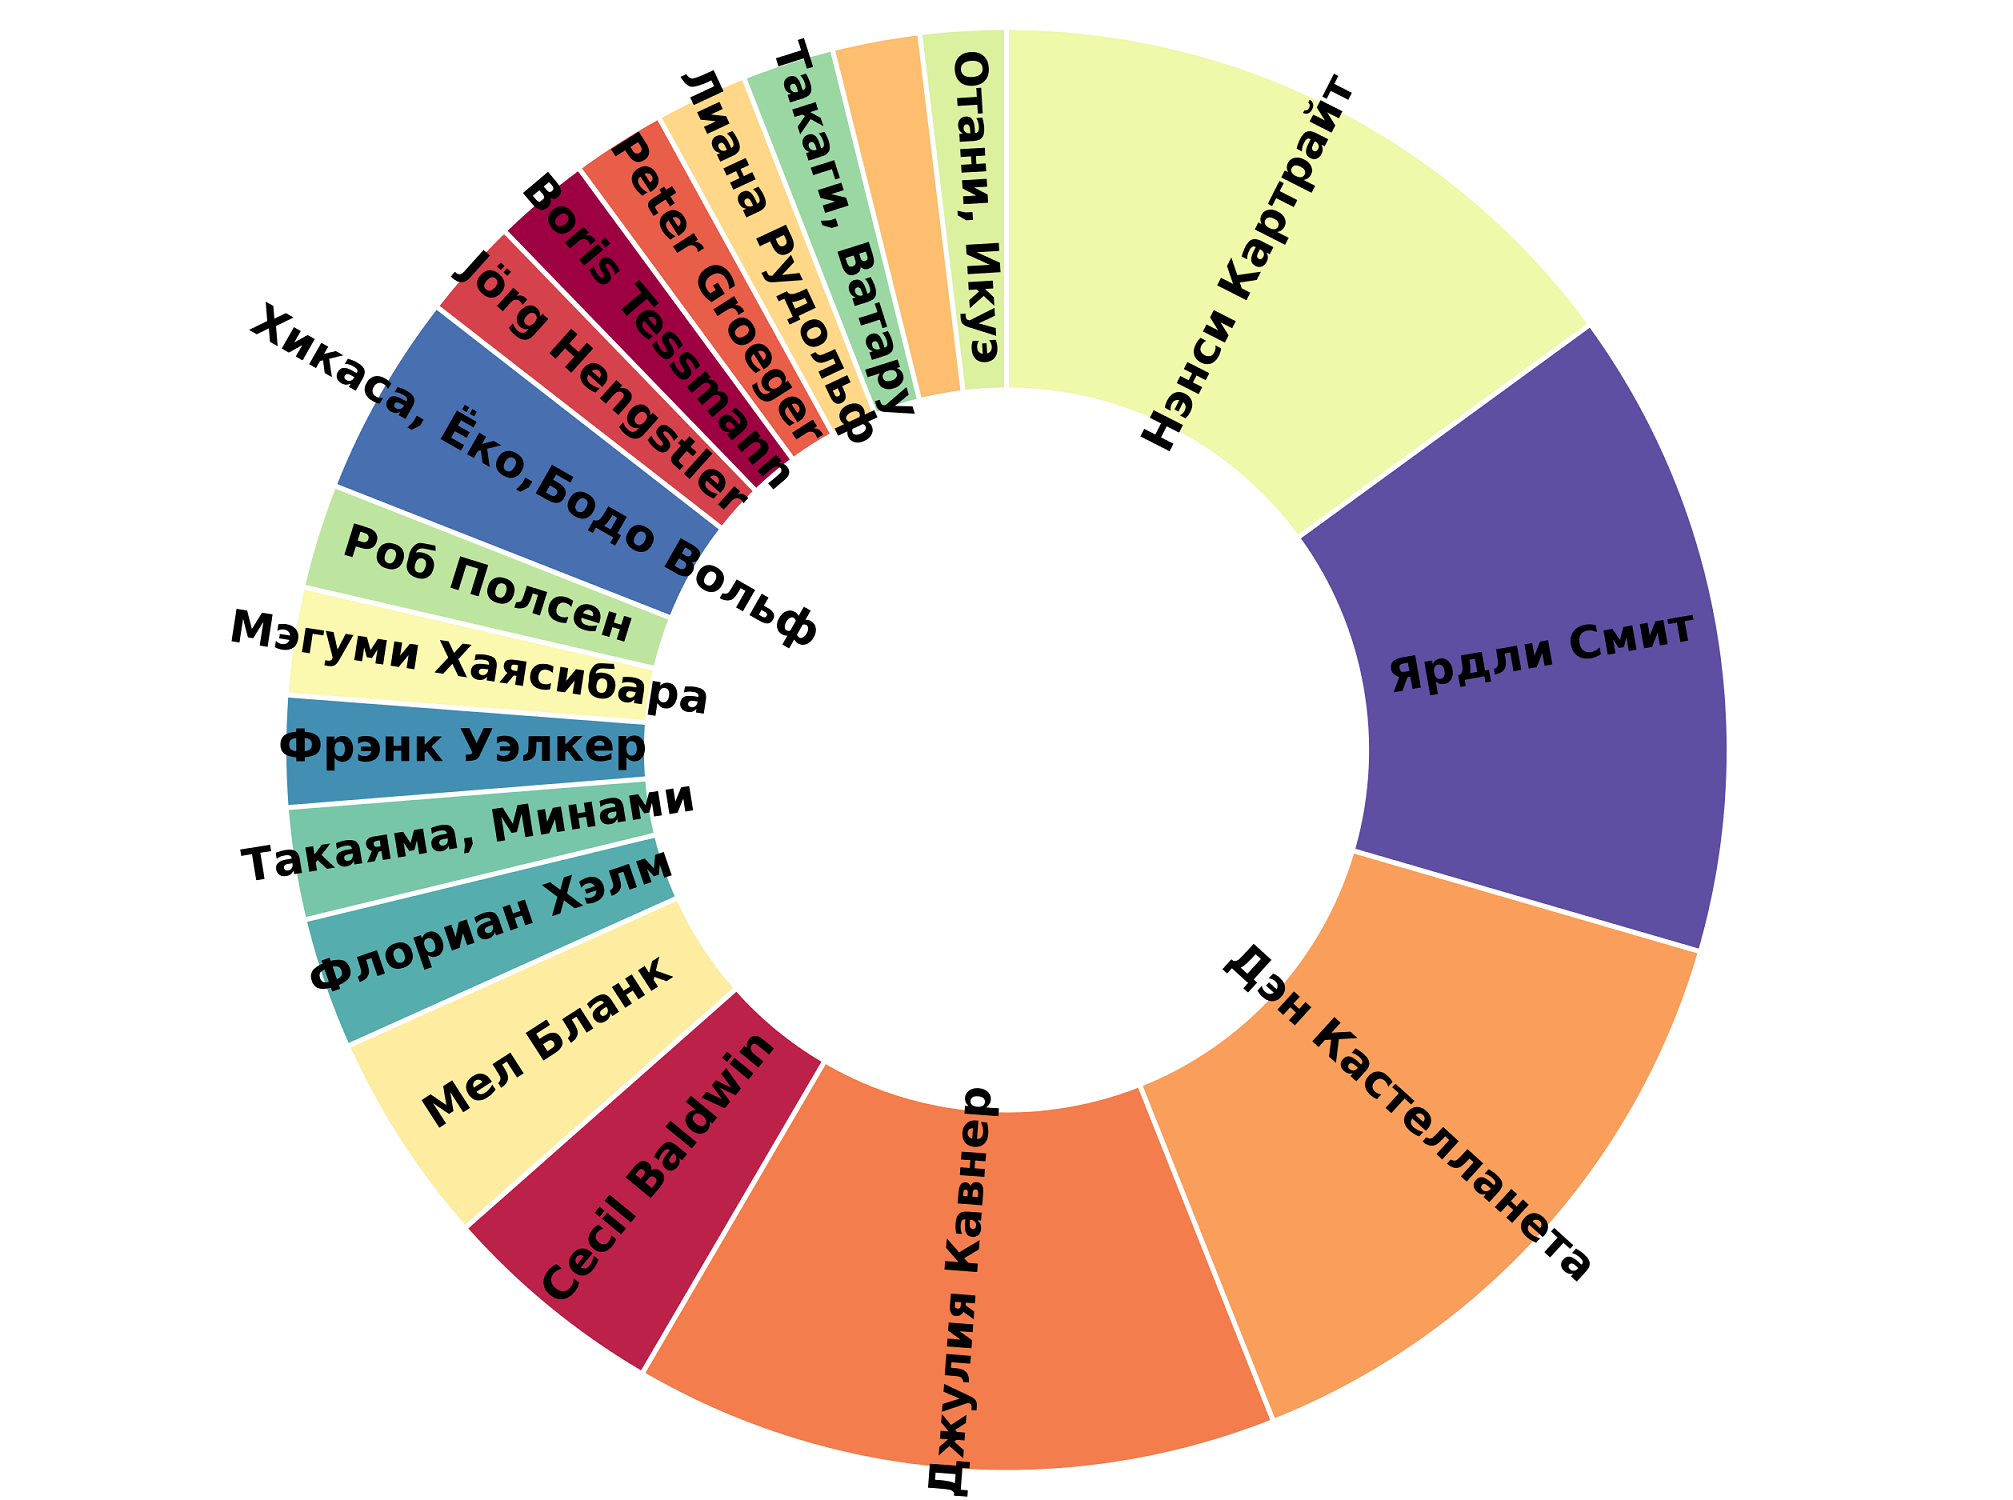
\includegraphics[width=1\linewidth]{./chapter/anime/actors-role-counts-sunburst-diagram-2021.png}}%
}%
    \caption[Круговая диаграмма числа ролей, озвученных различными сэйю, 2021 год.]{Диаграмма <<солнечные лучи>> числа ролей, озвученных различными актёрами, построенная в~2021 году с~помощью сервиса Rawgraphs (\href{https://app.rawgraphs.io}{https://app.rawgraphs.io}).}%
\label{fig:roles_piechart}%
\end{marginfigure}%


%\begin{figure*}[h!]
%    \index{График!Sunburst diagram!Количество ролей, озвученных разными актёрами}
%	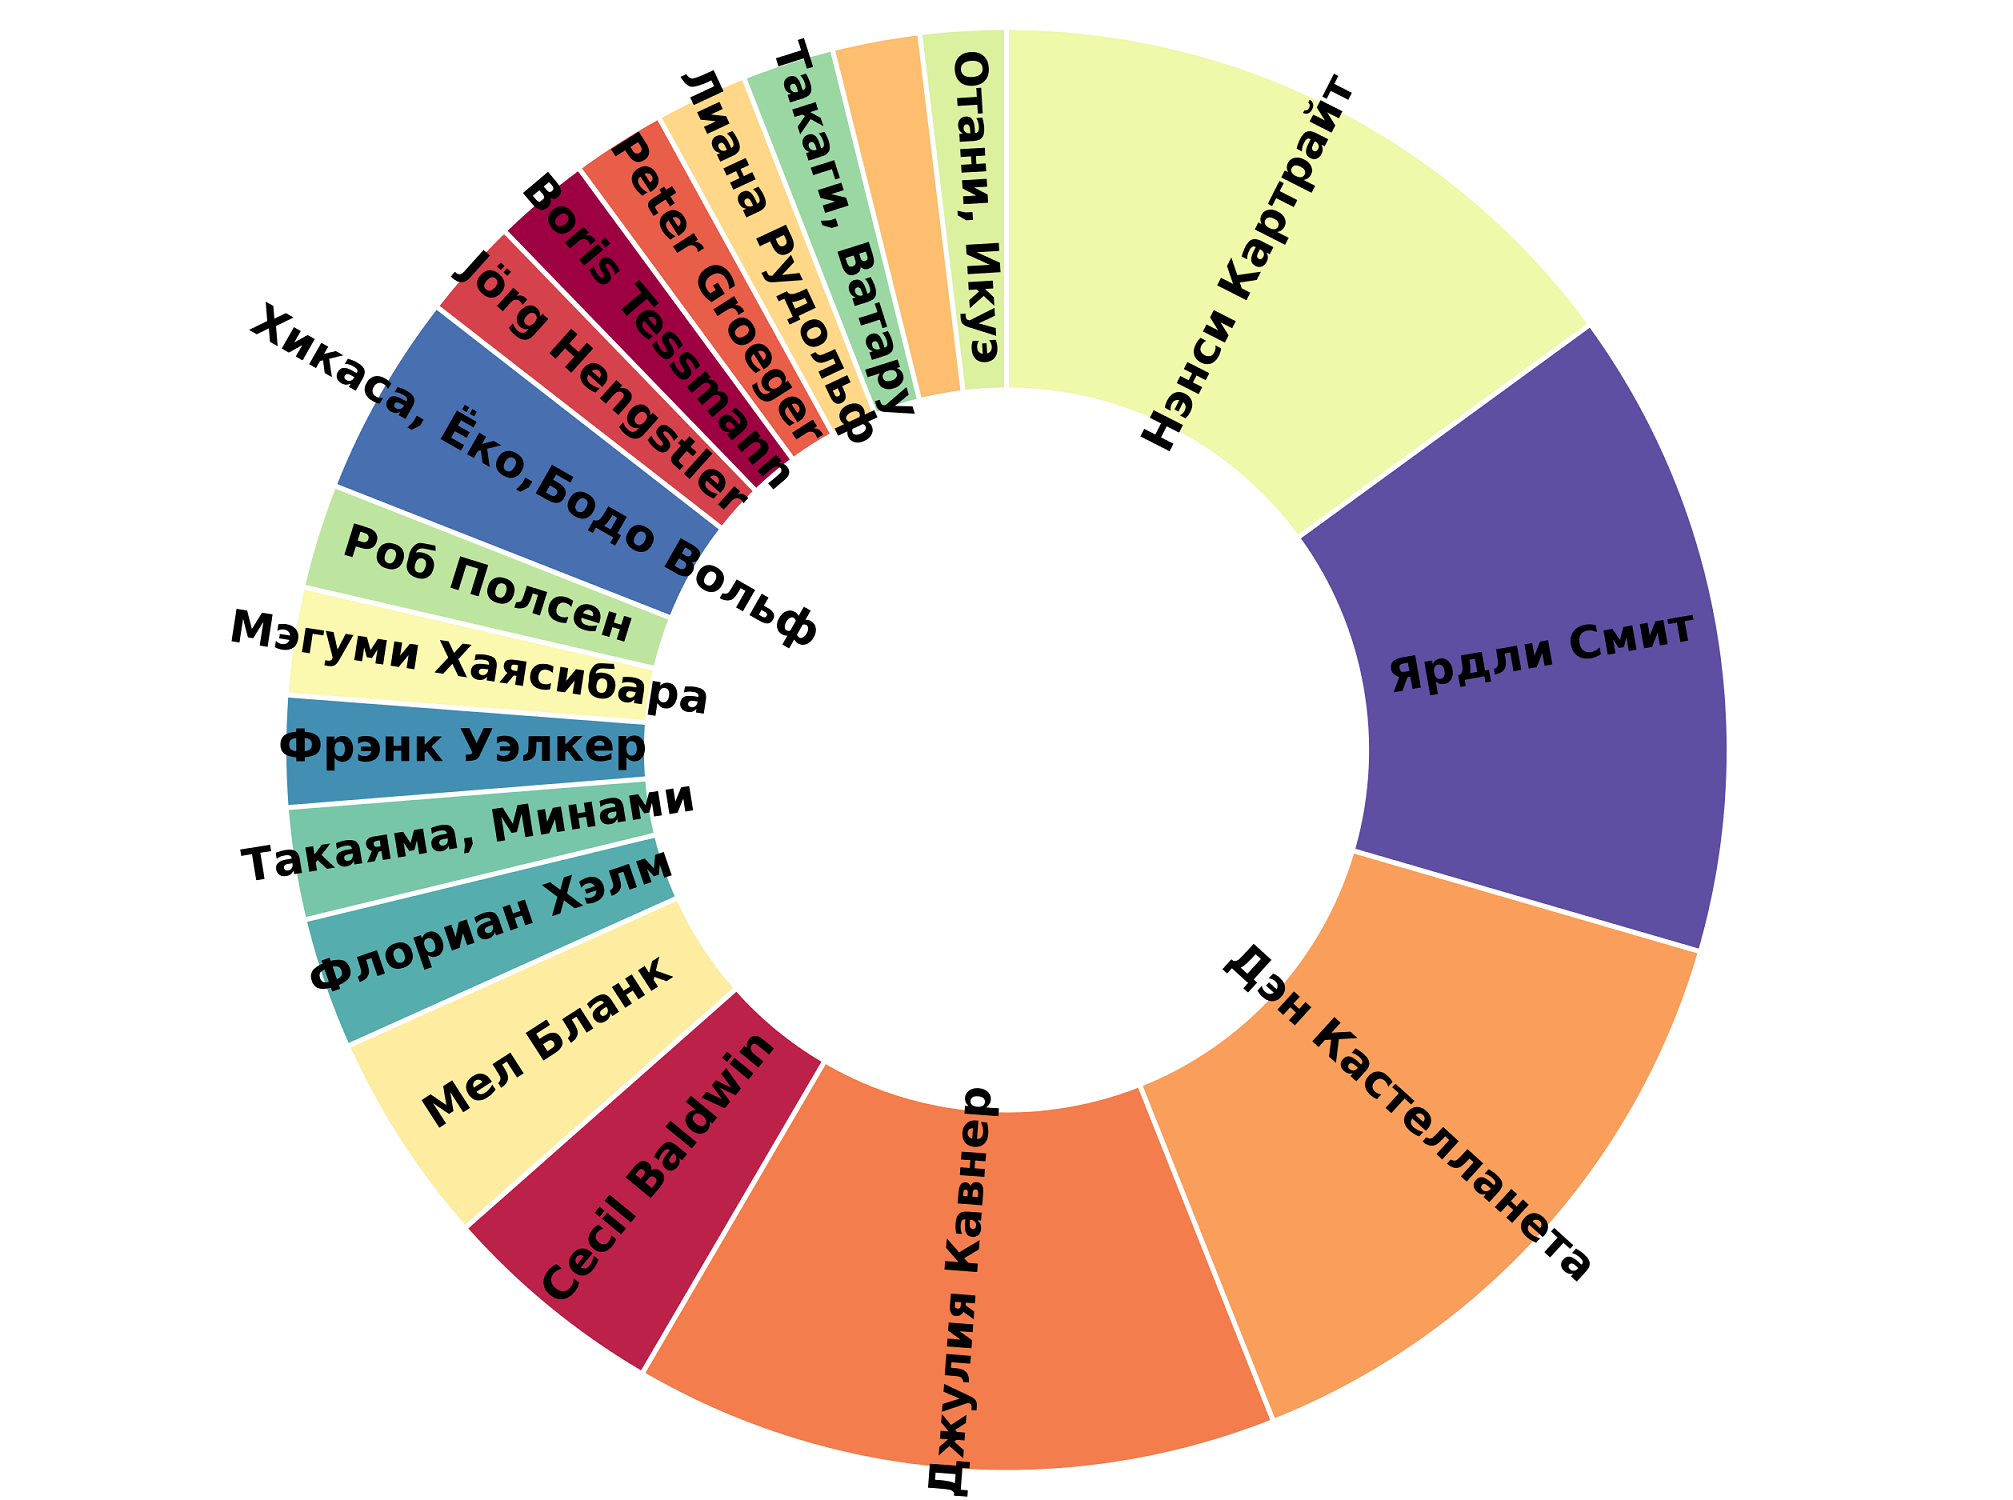
\includegraphics[width=0.7\linewidth]{./chapter/anime/actors-role-counts-sunburst-diagram-2021.png}
%	\caption[Круговая диаграмма числа ролей, озвученных различными сэйю, 2021 год.]{Диаграмма <<солнечные лучи>> числа ролей, озвученных различными актёрами, построенная в 2021 году с помощью сервиса Rawgraphs (\href{https://app.rawgraphs.io}{https://app.rawgraphs.io}).}%
%      \label{fig:roles_piechart}%
%\end{figure*}
Вспомним запрос~\ref{lst:seiyu_titles_sorted}, в котором говорилось о \num{2910} сэйю на Викиданных. Дело в том, что поиск производился только по актёрам озвучивания, связанным с аниме, поэтому результат оказался таким скромным. Если запросить информацию о всех актёрах озвучивания (то есть убрать ограничение на категорию аниме), то количество результатов может увеличиться в \num{5} раз (листинг~\ref{lst:voice_actors_list}). Значительный прирост числа результатов относительно запроса~\ref{lst:seiyu_titles_sorted} напоминает нам о том, что в индустрии озвучивания гораздо больше направлений, чем только аниме~--- например, озвучивание фильмов и видеоигр. Сэйю могут участвовать и в работе над такими проектами, и это нужно учитывать при формировании запросов. 

\begin{lstlisting}[ language=SPARQL, 
                    caption={\href{https://w.wiki/4aQt}{Получение списка актёров озвучки и числа озвученных ими проектов}\protect\footnotemark},
                    label=lst:voice_actors_list,
                    texcl 
                    ]
# Ordered list of actors according to the quantity of projects
# voiced by them
SELECT ?actor ?actorLabel (COUNT(?project) AS ?count)
WHERE
{
  ?project wdt:P725 ?actor.	# instance of voice actor
  SERVICE wikibase:label {bd:serviceParam wikibase:language "ru,en,ja"}
}
GROUP BY ?actor ?actorLabel
ORDER BY DESC(?count)       # order by number of voiced projects
\end{lstlisting}%
\footnotetext{Получено \num{3965} результатов в 2017 году и \num{14744} результата в 2021 году. Ссылка на SPARQL-запрос: \href{https://w.wiki/4aQt}{https://w.wiki/4aQt}}


Круговая диаграмма\index{Сервисы для анализа данных!Сервисы для визуализации данных!Rawgraphs} на рис.~\ref{fig:roles_piechart}~--- это один из вариантов визуализации данных, полученных с помощью скрипта~\ref{lst:voice_actors_list}. С помощью подобных диаграмм можно, например, оценить, какой актёр внёс наибольший вклад в развитие индустрии озвучивания.

\section{Указана ли дата публикации у аниме?}

Каждый ценитель японской анимации желает знать, в каком году вышло его любимое аниме. Викиданные располагают этой информацией не в полной мере. Напишем скрипт, который бы показывал количество аниме с незаполненным полем ''publication date'' (дата публикации) (листинг~\ref{lst:anime_no_pub_date}). То, что поле должно быть пустым, указано в шестой строке с помощью пустых квадратных скобок.

\lstset{numbers=left, firstnumber=1, frame=single}
\begin{lstlisting}[ language=SPARQL, 
                    caption={\href{https://w.wiki/4Hcz}{Получение списка аниме, у которых на Викиданных не указана дата выхода}\protect\footnotemark},
                    label=lst:anime_no_pub_date,
                    texcl 
                    ]
# List of anime the release date of which is empty
SELECT ?anime ?animeLabel
WHERE
{
    ?anime wdt:P31/wdt:P279* wd:Q1107;  # instance of anime
    FILTER NOT EXISTS { ?anime wdt:P577 [] }
    SERVICE wikibase:label{bd:serviceParam wikibase:language "ru,en,ja"}
}
\end{lstlisting}%
\footnotetext{Получено \num{237} результатов в 2017 году и \num{2940} результатов в 2021 году. Ссылка на SPARQL-запрос: \href{https://w.wiki/4Hcz}{https://w.wiki/4Hcz}}
\lstset{numbers=none}

На 2021 год из \num{4875} аниме на Викиданных (см. листинг~\ref{lst:all_anime_list}) у \num{2940}, а это \num{62}\%, не указана дата выхода. В 2017 году из \num{683} аниме на Викиданных только \num{237} (то есть \num{35}\%) не имели указанной даты выхода. Похоже, что, к сожалению, увеличение количества информации не всегда сопровождается сохранением её качества\footnote{Упражнение: напишите скрипт для вычисления доли аниме, у которых не указана дата публикации, относительно всех аниме на Викиданных. Сравните эту долю с долей за 2021 год (\num{62}\%) и сделайте вывод об изменении качества Викиданных.}.



\section{Анализ возраста, в котором сэйю озвучивают аниме}

Как и в любой другой профессии, у актёра озвучки есть возраст, 
когда он находится в~<<расцвете сил>> и может озвучить множество аниме. Использование SPARQL и внешних инструментов для анализа данных, таких как язык программирования Python\index{Языки программирования!Примеры языков программирования!Python}\footnote[][-1cm]{Язык Python~--- это интерпретируемый язык программирования, благодаря своей гибкости используемый для разнообразных задач. Его можно применять в том числе и для работы с Викиданными: например, в разделе~\ref{ch:bots} (с.~\pageref{ch:bots}) описан процесс создания программных ботов для Викиданных.}, может позволить оценить такой возраст на основе информации из Викиданных.

Чтобы получить исходные данные для исследования, необходимо выполнить три SPARQL-скрипта и экспортировать результаты их выполнения в формате .csv\footnote[][-0.3cm]{CSV (comma-separated values)~--- это формат представления табличных данных, в котором таблица хранится в виде последовательности строк текста. Эти строки содержат значения полей таблицы, разделённые запятыми.}. CSV-файлы затем используются в скрипте на языке Python, который генерирует выходной график. Запускать программы на Python можно, например, на платформе Google Colaboratory\footnote[][0.2cm]{Google Colaboratory (Colab)~--- это облачная среда разработки от компании Google, в которой можно создавать и запускать скрипты на языке программирования Python, а также делиться результатами своей работы с другими людьми. Также этот сервис удобен тем, что предоставляет вычислительные мощности~--- как обычные процессоры, так и видеокарты для, например, работы с нейронными сетями. Сервис доступен по ссылке \href{https://colab.research.google.com}{https://colab.research.google.com}.}.

\newpage
Получить список всех зарегистрированных в Викиданных сэйю и их дат рождения 
можно двумя способами (листинги~\ref{lst:seiyu_bd_w_service} и \ref{lst:seiyu_bd_w_rdfs}): 
с помощью команды \lstinline|SERVICE|\index{SPARQL!SERVICE!Получение дат рождения сэйю} 
и с помощью конструкции \lstinline|rdfs:label|. 
Различия между скриптами (листинги~\ref{lst:seiyu_bd_w_service} и \ref{lst:seiyu_bd_w_rdfs}) заключаются в~том, что:
%
\begin{itemize}%[noitemsep,topsep=0pt]
    \item метка (имя) сэйю в первом случае получается с помощью переменной \lstinline|?seiyuLabel| 
        (в~таком случае нужно указать команду \lstinline|SERVICE| для установки языков, на котором будут возвращены имена), 
        а во втором~--- с помощью конструкции \lstinline|rdfs:label|;
    \item в первом варианте скрипта необходимо указывать \lstinline|?seiyuLabel| 
        как параметр \lstinline|GROUP BY|\index{SPARQL!GROUP BY!Получение дат рождения сэйю}, чтобы связать объекты сэйю и их метки.
\end{itemize}

% # Get list of all seiyu objects, their names and birth dates
\begin{fullwidth}
%
\noindent\begin{minipage}[]{.49\linewidth}
\begin{lstlisting}[ language=SPARQL, breaklines=false, numbers=none,
                    caption={Получение списка дат рождения сэйю с помощью \lstinline|SERVICE|\protect\footnotemark},
                    label=lst:seiyu_bd_w_service,
                    texcl,
                    escapechar=!
                    ]
SELECT ?seiyu ?seiyuLabel ?bDate
WHERE {
  ?anime (wdt:P31/(wdt:P279*)) wd:Q1107;
    wdt:P725 ?seiyu.       
  ?seiyu wdt:P569 ?bDate. 
  SERVICE wikibase:label {bd:serviceParam wikibase:language "ru,en,ja"}
}
GROUP BY ?seiyu ?seiyuLabel ?bDate
\end{lstlisting}%
    \footnotetext[30]{Получено \num{2515} результатов в 2021 году. SPARQL-запрос: \href{https://w.wiki/4FPq}{https://w.wiki/4FPq}}
\end{minipage}%
%just a break for lines between two columns of listings
\hfill
\begin{minipage}[]{.5\linewidth}
\begin{lstlisting}[ language=SPARQL, breaklines=true, numbers=none,
                    caption={Получение списка дат рождения сэйю с помощью \lstinline|rdfs:label|\protect\footnotemark},
                    label=lst:seiyu_bd_w_rdfs,
                    texcl,
                    escapechar=!
                    ]
SELECT ?seiyu (SAMPLE(?seiyu) AS ?seiyuLabel) ?bDate
WHERE {
  ?anime (wdt:P31/(wdt:P279*)) wd:Q1107;
    wdt:P725 ?seiyu.      # seiyu is anime voice actor
  ?seiyu wdt:P569 ?bDate. # has a birthday 
  ?seiyu rdfs:label ?label.
}
GROUP BY ?seiyu ?bDate
\end{lstlisting}%
    \footnotetext[31]{Получено \num{2515} результатов в 2021 году. SPARQL-запрос: \href{https://w.wiki/4FPn}{https://w.wiki/4FPn}}
\end{minipage}
\end{fullwidth}%








\newpage
Получим список всех зарегистрированных в Викиданных 
аниме и дат их выхода (листинг~\ref{lst:all_anime_releases})\marginnote[1cm]{%
%
Упражнение: визуализируйте результаты работы скрипта~\ref{lst:all_anime_releases}.\\
Усложните задачу~--- добавьте на график даты окончания показа сериалов.}.

\begin{lstlisting}[ language=SPARQL, 
                    caption={\href{https://w.wiki/4ENc}{Получение дат выхода аниме}\protect\footnotemark},
                    label=lst:all_anime_releases,
                    texcl 
                    ]
# Get all anime objects, their names and release dates
SELECT ?anime ?animeLabel ?animePubDate ?animeSeriesStartDate
WHERE {
  ?anime (wdt:P31/(wdt:P279*)) wd:Q1107.                # object of anime/subclass
  OPTIONAL { ?anime wdt:P577 ?animePubDate. }           # release date of a movie
  OPTIONAL { ?anime wdt:P580 ?animeSeriesStartDate. }   # start date of a series
  SERVICE wikibase:label{bd:serviceParam wikibase:language "ru,en,ja"}
}
\end{lstlisting}%
\footnotetext{Получено \num{5264} результата в 2021 году. Ссылка на SPARQL-запрос: \href{https://w.wiki/4ENc}{https://w.wiki/4ENc}}

Обратите внимание, что запрос~\ref{lst:all_anime_releases} получает не только  \wdProperty{577}{даты выхода полнометражных аниме}, но и \wdProperty{580}{даты начала показа сериалов}. 

Получим ссылки между объектами сэйю и аниме, которые они озвучивали (листинг~\ref{lst:link_anime_seiyu}).

\begin{lstlisting}[ language=SPARQL, 
                    caption={\href{https://w.wiki/4ELh}{Получение ссылок между сэйю и аниме}\protect\footnotemark},
                    label=lst:link_anime_seiyu,
                    texcl 
                    ]
# List of links between seiyu and anime where they are involved in
SELECT DISTINCT ?item ?itemLabel ?link ?itemType
WHERE
{
  VALUES ?toggle { true false }
  ?anime  wdt:P31/wdt:P279* wd:Q1107;   # instance of anime/subclass
          wdt:P725 ?seiyu.              # list seiyu who acted in this anime
  
  BIND(IF(?toggle,?anime,?seiyu) AS ?item).                 # anime/seiyu object
  BIND(IF(?toggle,?animeLabel,?seiyuLabel) AS ?itemLabel).  # anime/seiyu labels link
  BIND(IF(?toggle,?seiyu,?anime) AS ?link).                 # seiyu/anime link
  BIND(IF(?toggle,?seiyu,"seiyu") AS ?itemType).
  SERVICE wikibase:label{bd:serviceParam wikibase:language "ru,en,ja"}
}
\end{lstlisting}%
\footnotetext{Получено \num{27092} результата в 2021 году. Ссылка на SPARQL-запрос: \href{https://w.wiki/4ELh}{https://w.wiki/4ELh}}
% [40][-2cm]

Результат анализа удобно представить в виде гистограммы. Для её построения воспользуемся средствами таких библиотек для Python, как \href{https://ru.wikipedia.org/wiki/Pandas}{Pandas}\footnote[][-5cm]{pandas~--- библиотека для языка Python, предоставляющая различные функции для обработки табличных данных. \href{https://ru.wikipedia.org/wiki/Pandas}{https://ru.wikipedia.org/wiki/Pandas}, 2021}\index{Языки программирования!Библиотеки для языков программирования!Pandas} и \href{https://ru.wikipedia.org/wiki/Matplotlib}{Matplotlib}\footnote[][-2.7cm]{Matplotlib~--- библиотека для языка Python, предназначенная для построения разнообразных графиков и диаграмм. \href{https://ru.wikipedia.org/wiki/Matplotlib}{https://ru.wikipedia.org/wiki/Matplotlib}, 2021}\index{Языки программирования!Библиотеки для языков программирования!Matplotlib}. Код скрипта, создающего гистограмму, опубликован на сервисе \href{https://git.io/J1UGA}{GitHub}\footnote{Ссылка на скрипт в проекте wd\_book на GitHub: \href{https://git.io/J1UGA}{https://git.io/J1UGA}}.

В результате получим гистограмму, по оси абсцисс которой отложен возраст в годах, а по оси ординат~--- суммарное количество ролей, озвученных всеми сэйю такого возраста. Получившаяся гистограмма представлена на рис.~\ref{fig:Seiyu_age_hist_RU}. 

\index{График!Histogram!Число аниме, озвученных сэйю разных возрастов}
\begin{figure*}[h!]

    \setlength{\fboxsep}{0pt}%
    \setlength{\fboxrule}{1pt}%
    \fcolorbox{gray}{gray}{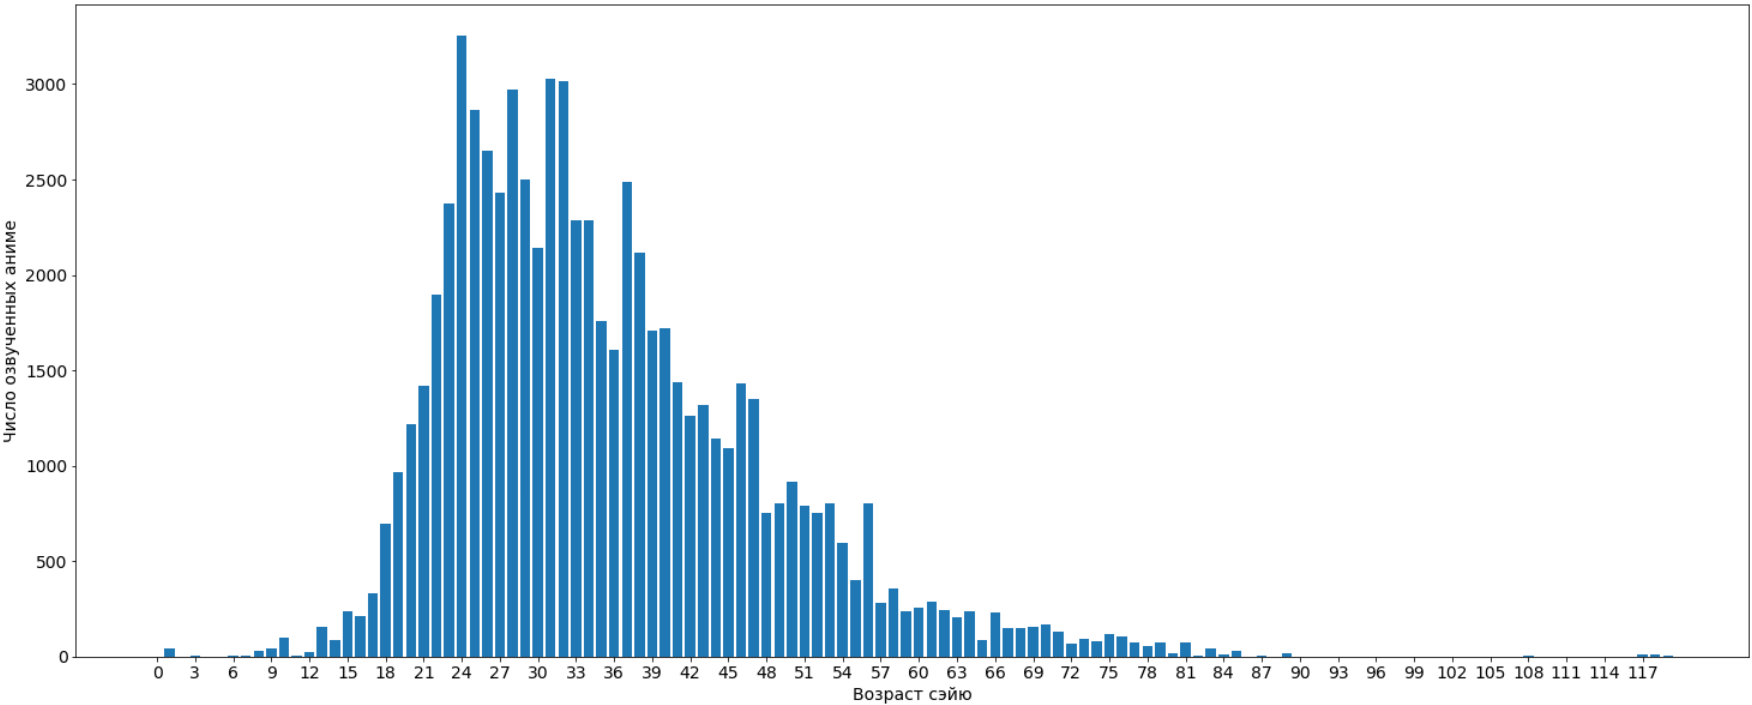
\includegraphics[width=\linewidth]{./chapter/anime/Seiyu_age_hist_RU.png}}
	\caption[Гистограмма с числом аниме, озвученных сэйю разных возрастов, 2021 года.]{Гистограмма с числом аниме, озвученных сэйю разных возрастов, 2021 год. Гистограмма построена на~основе данных, полученных с помощью запросов~\protect\ref{lst:seiyu_bd_w_service} (или~\protect\ref{lst:seiyu_bd_w_rdfs}), \protect\ref{lst:all_anime_releases} и \protect\ref{lst:link_anime_seiyu}.}%
    \label{fig:Seiyu_age_hist_RU}%
\end{figure*} 
 	
Отметим следующий забавный факт: в Викиданных нашлись случаи, когда сэйю родился позже, чем вышло аниме с его участием. Вероятно, это связано с отсутствием информации в Викиданных о втором сезоне/перезапуске аниме. Например, на 2021 год такая ситуация наблюдается для аниме \wdqName{Sazae-san}{11304591} и сэйю \wdqName{Нобунага Симадзаки}{5968283}: сэйю родился в 1988 году, а дата выхода аниме с его участием~--- 1969 год.

\section{Упражнения}

\begin{enumerate}
    \item Вывести 10 самых популярных аниме, вышедших на экраны в текущем году. Популярность оценить по числу статей в разных языковых разделах. Для подсчёта числа статей об объекте Викиданных используйте SPARQL-конструкцию \lstinline|wikibase:sitelinks|. Например, если статья про аниме есть в трёх Википедиях на русском, английском и испанском языках, то его популярность равна трём. 
    \item Вывести пять аниме, в которых задействовано самое большое число сэйю-женщин.
    \item Построить пузырьковую диаграмму (BubbleChart) распределения аниме по жанрам (сколько аниме в каждом жанре), воспользовавшись свойством \wdProperty{279}{<<подкласс>>}.
    \item Отметить на карте места рождения сэйю.
    \item Построить гистограмму или пузырьковую диаграмму национальностей сэйю.
    \item Построить гистограмму количества вышедших аниме по годам или количества сэйю по~годам рождения.
    \item Построить гистограммы, аналогичные рисунку~\ref{fig:Seiyu_age_hist_RU}, но с учётом пола сэйю (одну для~мужчин, другую для женщин).
\end{enumerate}
